\documentclass[12pt]{article}
\usepackage{graphicx}
\usepackage{hyperref}
\usepackage{geometry}
\geometry{margin=1in}

\title{Global Migration Network Analysis: Data Science and Network Science Approaches}
\author{Jaswinder Singh (ID: 12340970) \\ Aditya Yadav \\ Dipanjan Mondal}
\date{April 2026}

\begin{document}
\maketitle

\section{Project Aim}
The aim of this project was to analyze global migration flows using advanced data science and network science techniques. We set out to:
\begin{itemize}
  \item Clean and integrate international migration datasets
  \item Construct dynamic migration networks
  \item Detect communities and analyze their evolution
  \item Model migration determinants using regression
  \item Build interactive dashboards for exploration
\end{itemize}

\section{Data Collection}
\textbf{Primary Source:} United Nations Department of Economic and Social Affairs (UN DESA) International Migrant Stock 2024 Excel file (undesa\_pd\_2024\_ims\_stock\_by\_sex\_destination\_and\_origin.xlsx)\\
\textbf{Auxiliary Data:} World Bank (GDP, population, unemployment), UNDP, UCDP (conflict), and other open sources (where available)\\
\textbf{Collaboration:} Integrated and compared with the open-source Nodes\_And\_Nations repository for advanced pipelines and validation

\section{Data Preparation \& Cleaning}
\begin{itemize}
  \item Parsed the UN DESA Excel into long-format bilateral migration flows (country-to-country, by year)
  \item Cleaned and filtered out non-country and aggregate rows
  \item Merged auxiliary factor data (where available) on (country, year)
  \item Handled missing values and harmonized country codes
  \item Exported cleaned datasets for analysis
\end{itemize}

\section{Network Construction \& Centrality}
\begin{itemize}
  \item Built 8 dynamic directed migration networks (snapshots: 1990--2024/2025)
  \item Nodes: countries; Edges: migration flows (weighted)
  \item Computed centrality metrics: in-degree, out-degree, betweenness, PageRank
  \item Exported centrality CSVs for each snapshot
\end{itemize}

\section{Community Detection \& Temporal Analysis}
\begin{itemize}
  \item Applied Louvain, Leiden, and Girvan-Newman algorithms to detect communities in each network snapshot
  \item Calculated modularity Q for each method and year
  \item Compared partitions using Normalized Mutual Information (NMI), Adjusted Rand Index (ARI), and Jaccard drift
  \item Analyzed community stability and boundary nodes over time
\end{itemize}

\section{Regression Analysis}
\begin{itemize}
  \item Merged centrality and factor data for regression modeling
  \item Fitted baseline and full OLS models (log-migrants $\sim$ log-population, log-GDP, conflict, etc.)
  \item Compared models using $R^2$, AIC, and VIF (Variance Inflation Factor)
  \item Exported coefficient tables and diagnostics
\end{itemize}

\section{Dashboarding \& Visualization}
Generated dashboard-ready CSVs and Power BI screenshot exports for:
\begin{itemize}
  \item Executive overview
  \item Top migration corridors
  \item Temporal trends
  \item Community structure
  \item Regression diagnostics
\end{itemize}
A Power BI build spec was provided for interactive dashboard recreation.

\section{Algorithms Used}
\begin{itemize}
  \item \textbf{Network Construction:} NetworkX DiGraph, edge aggregation
  \item \textbf{Centrality:} in-degree, out-degree, betweenness, PageRank (NetworkX)
  \item \textbf{Community Detection:} Louvain (python-louvain), Leiden (leidenalg, igraph), Girvan-Newman (NetworkX)
  \item \textbf{Partition Comparison:} NMI, ARI (scikit-learn), Jaccard drift
  \item \textbf{Regression:} OLS (statsmodels), VIF analysis
  \item \textbf{Visualization:} matplotlib, seaborn, Power BI
\end{itemize}

\section{Workflow Summary}
\begin{enumerate}
  \item Data collection from UN DESA and APIs
  \item Data cleaning and integration
  \item Network construction for each snapshot
  \item Centrality and community analysis
  \item Regression modeling
  \item Dashboard and report generation
\end{enumerate}

\section{Collaboration \& Validation}
Collaborated with the Nodes\_And\_Nations open-source project for pipeline validation and advanced analytics. Compared outputs and algorithms for robustness.

\section{Key Results}
\begin{itemize}
  \item Identified top migration corridors and hubs
  \item Detected persistent and shifting communities
  \item Regression models explained migration determinants with high accuracy (best $R^2 \approx 0.95$)
  \item Produced reproducible, dashboard-ready outputs
\end{itemize}

\section{Screenshots}
\begin{figure}[h!]
  \centering
  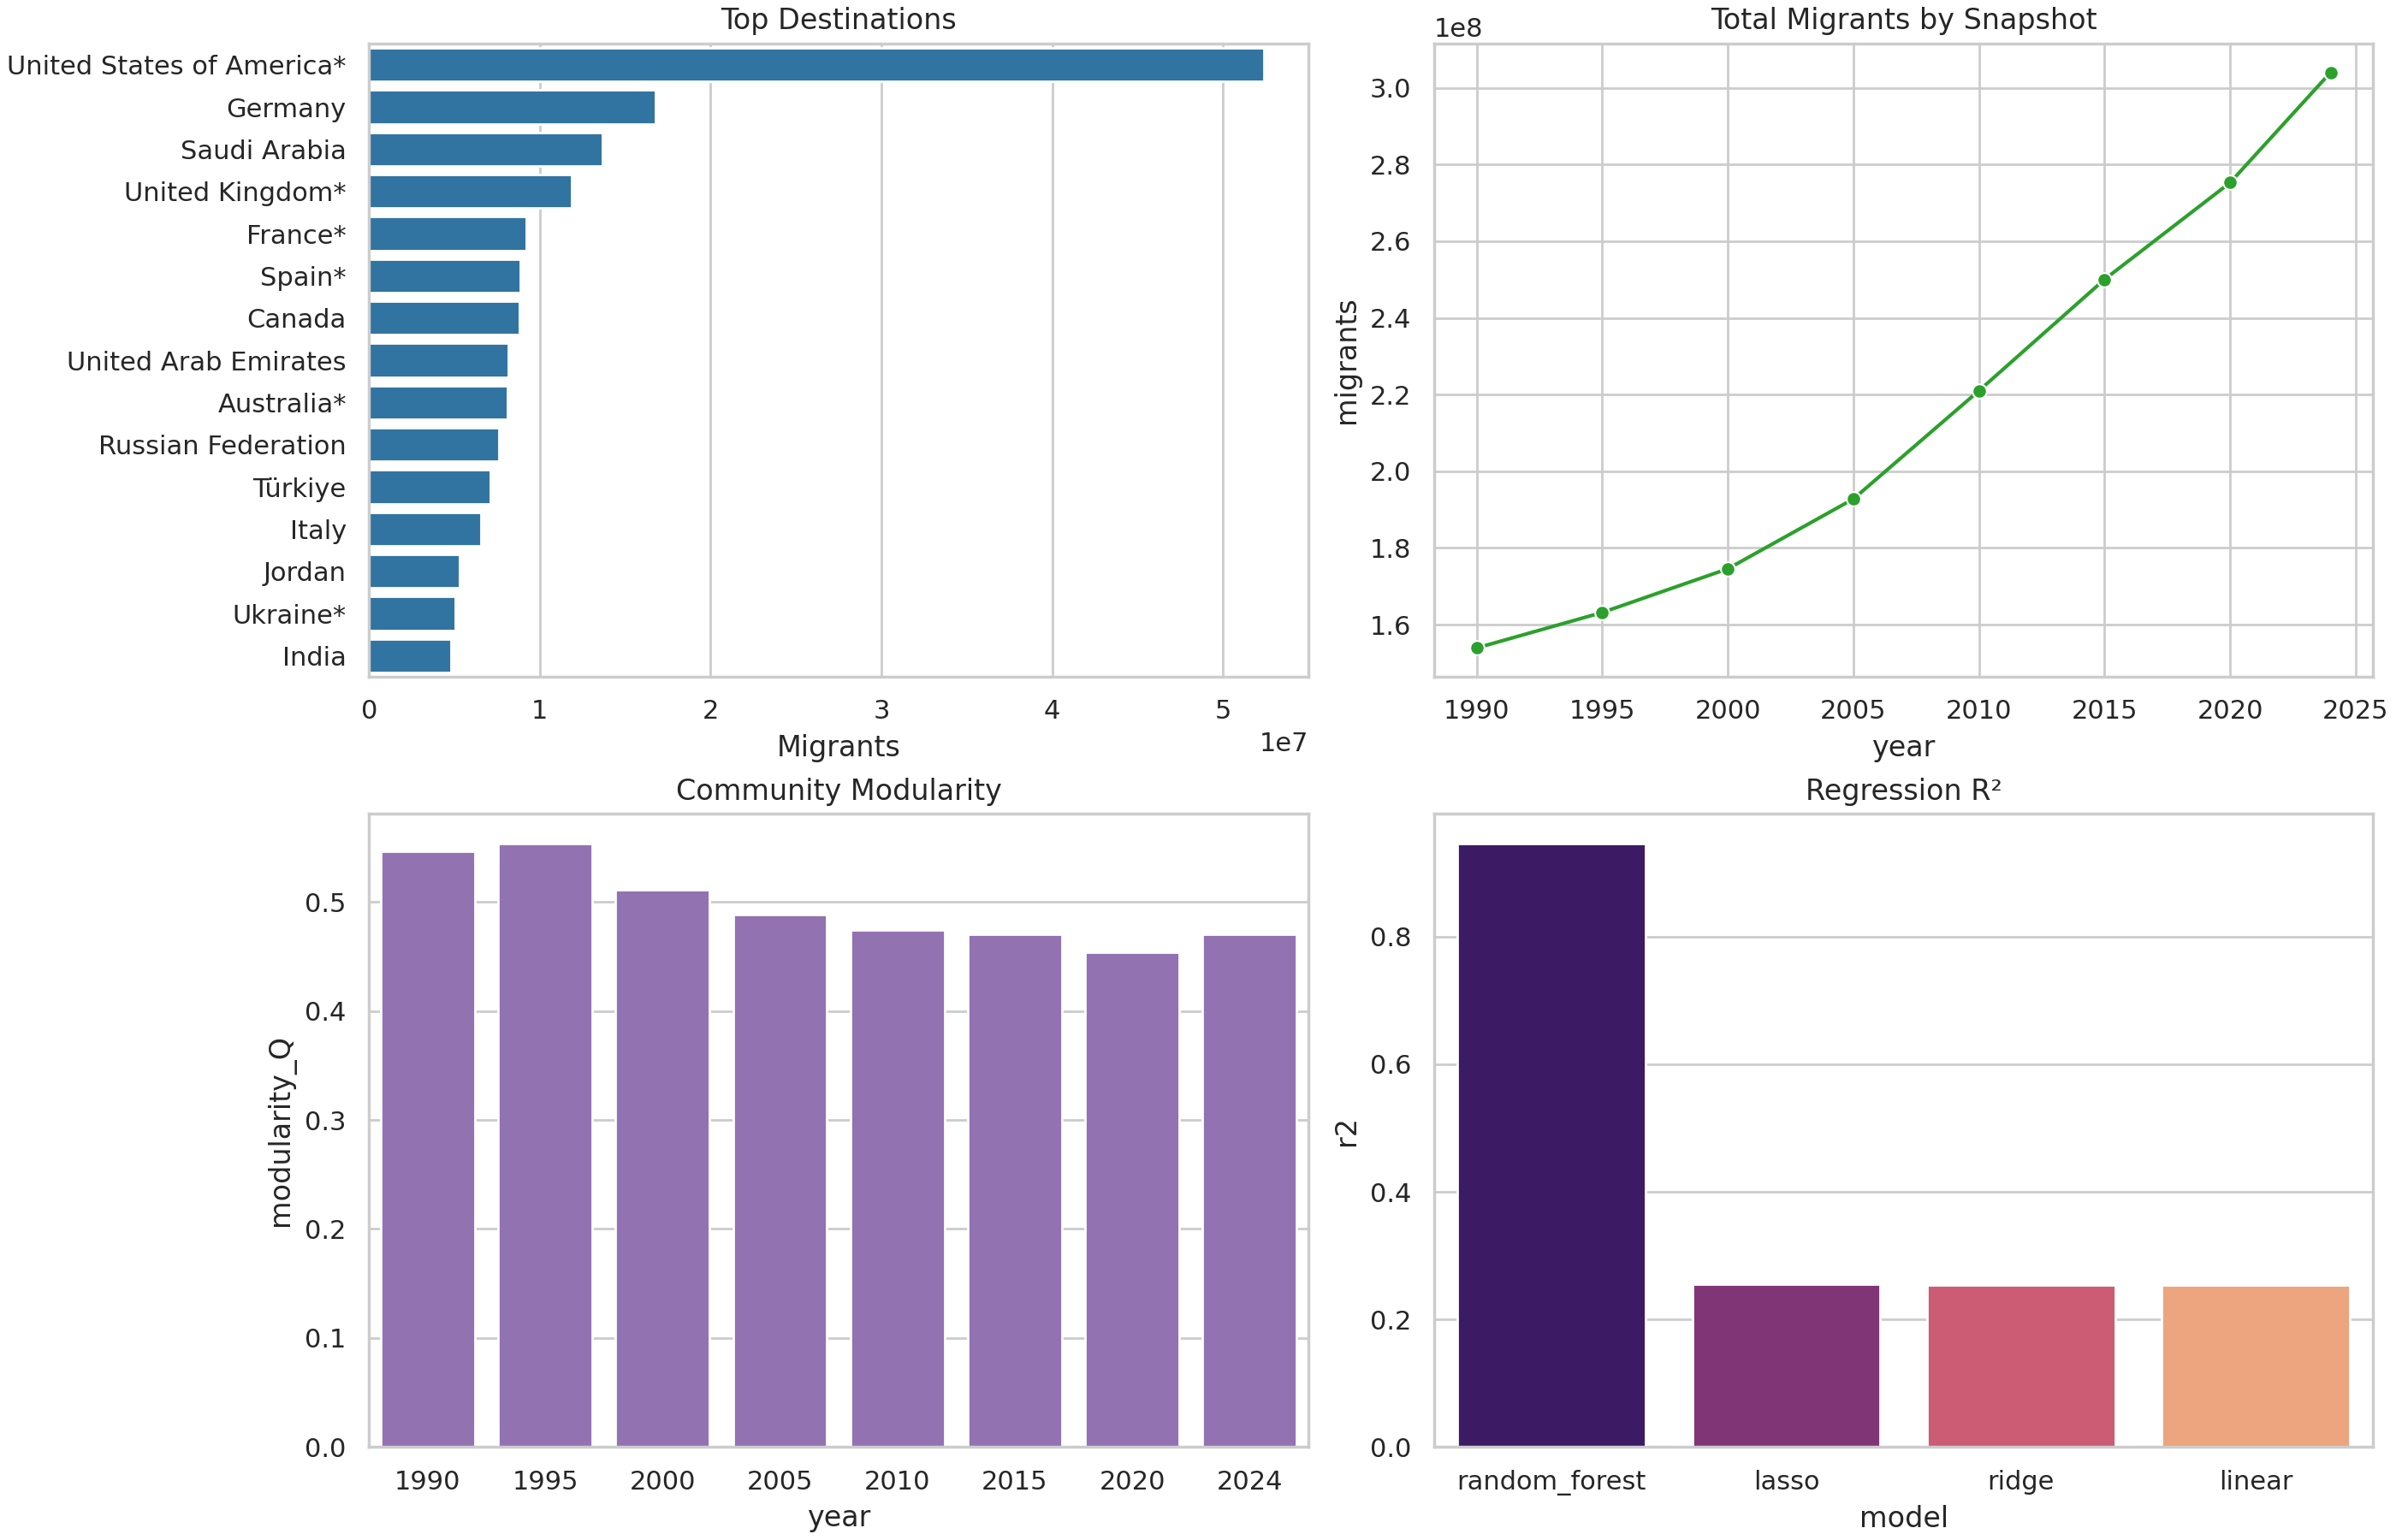
\includegraphics[width=0.8\textwidth]{deliverables_outputs/powerbi_exports/screenshots/dashboard_01_overview.png}
  \caption{Executive Overview Dashboard}
\end{figure}

\begin{figure}[h!]
  \centering
  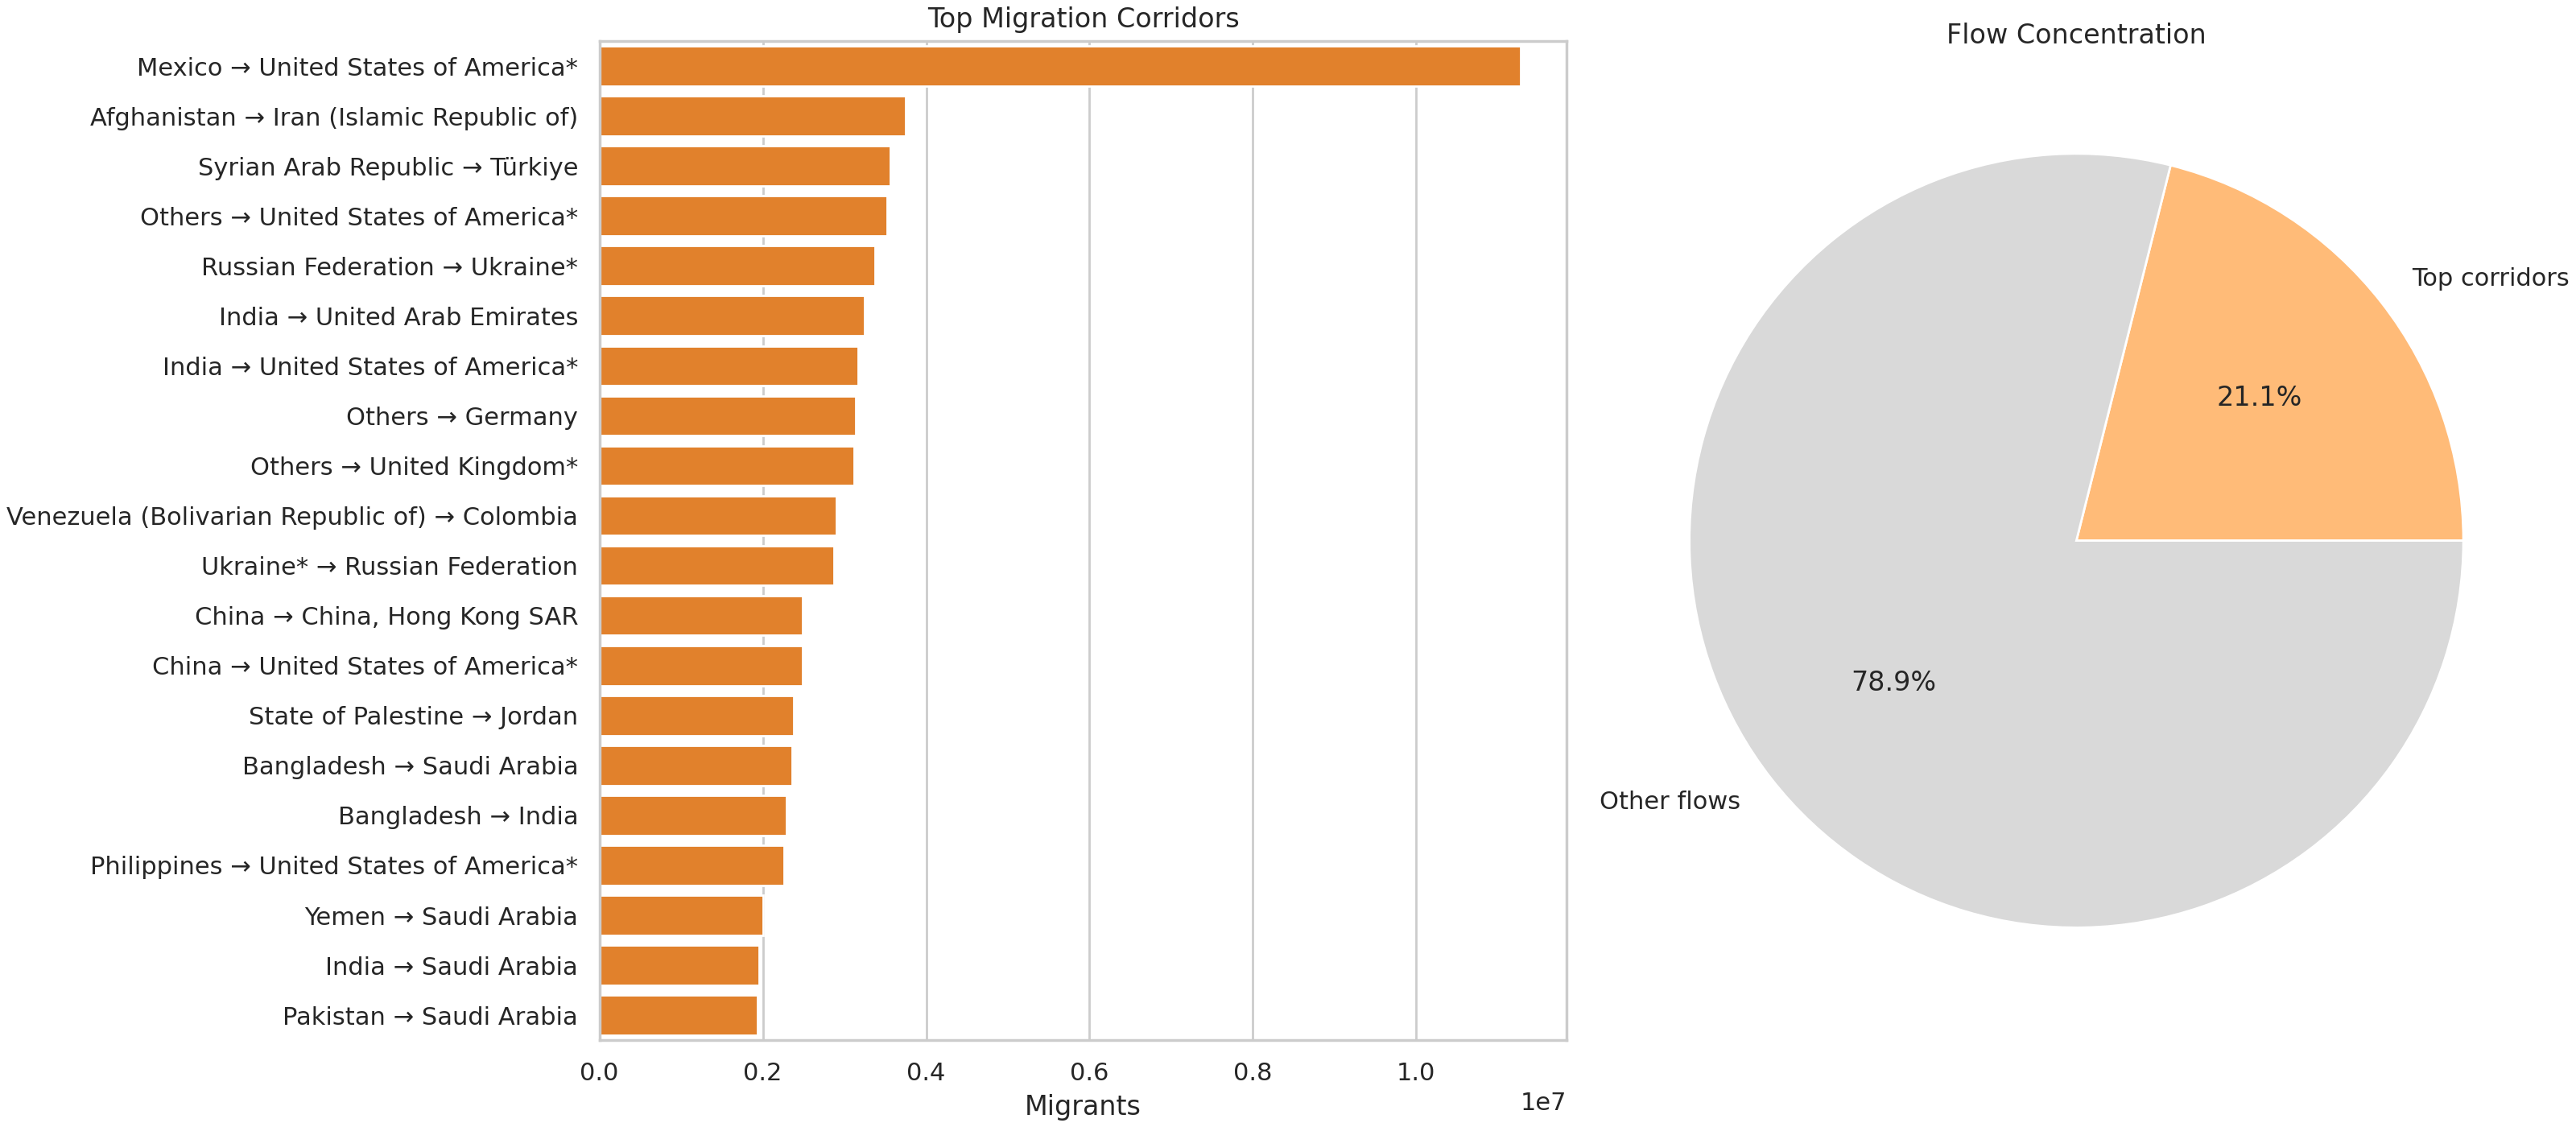
\includegraphics[width=0.8\textwidth]{deliverables_outputs/powerbi_exports/screenshots/dashboard_02_corridors.png}
  \caption{Top Migration Corridors}
\end{figure}

\begin{figure}[h!]
  \centering
  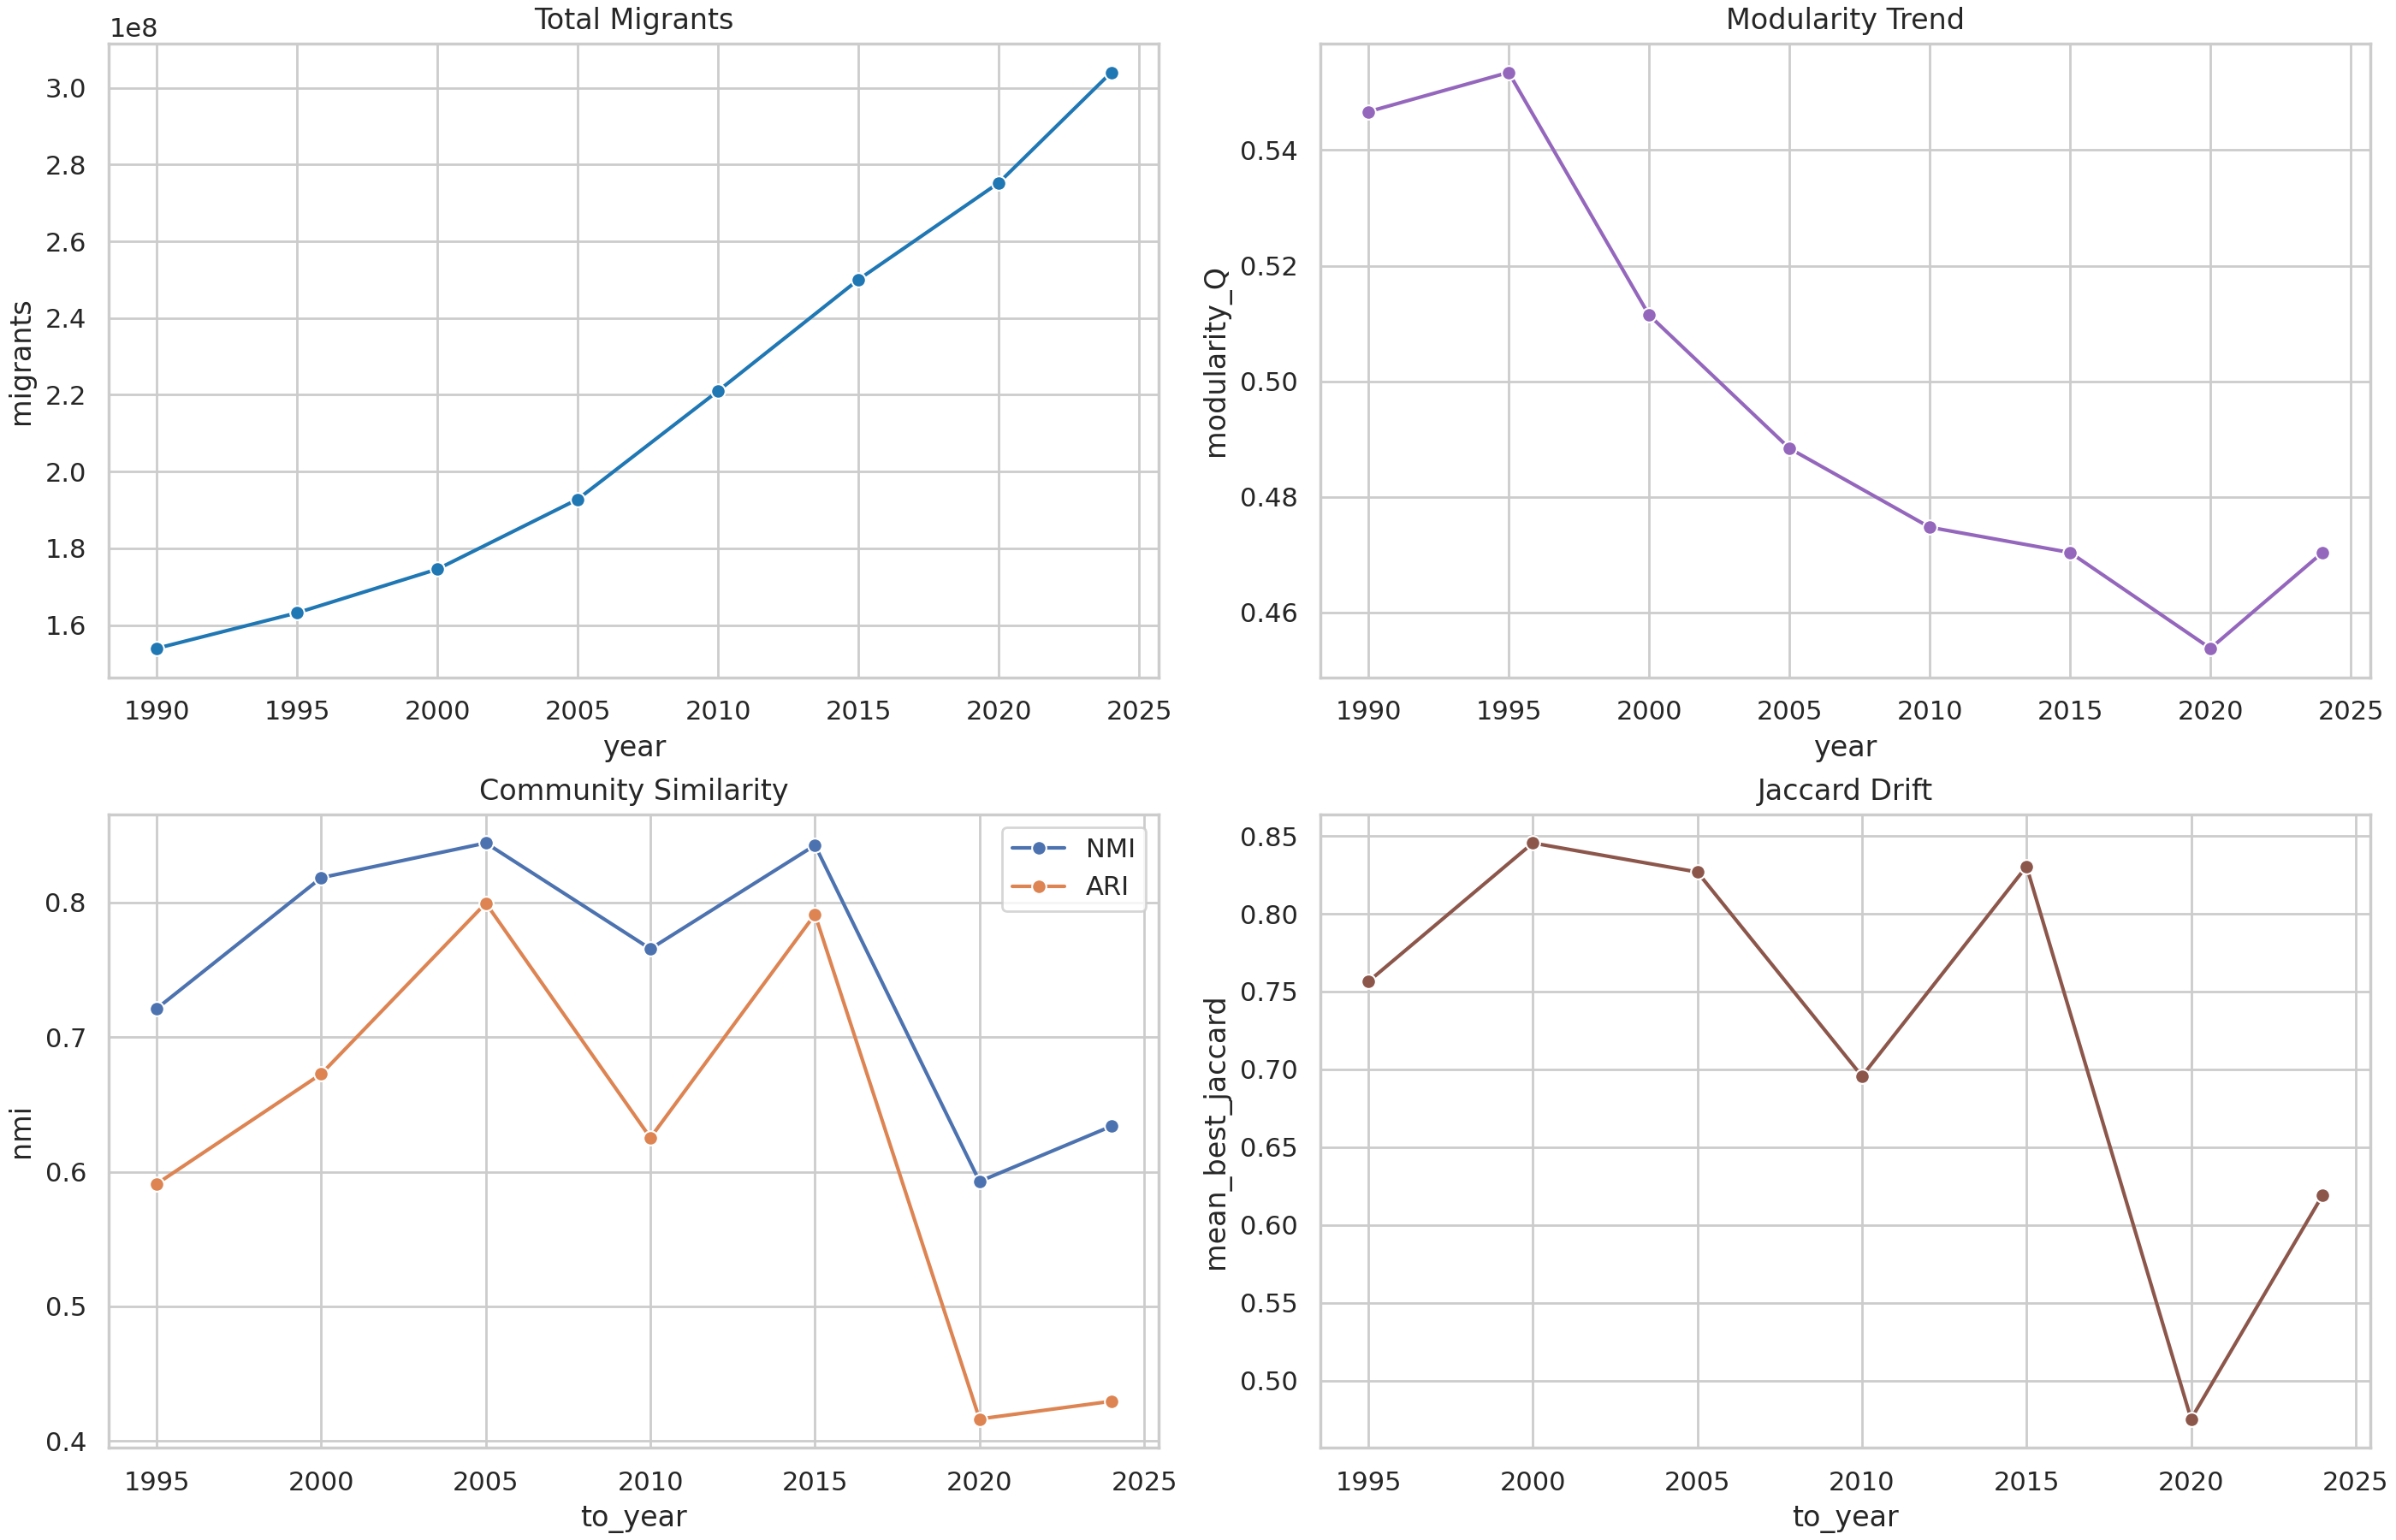
\includegraphics[width=0.8\textwidth]{deliverables_outputs/powerbi_exports/screenshots/dashboard_03_temporal.png}
  \caption{Temporal Trends}
\end{figure}

\begin{figure}[h!]
  \centering
  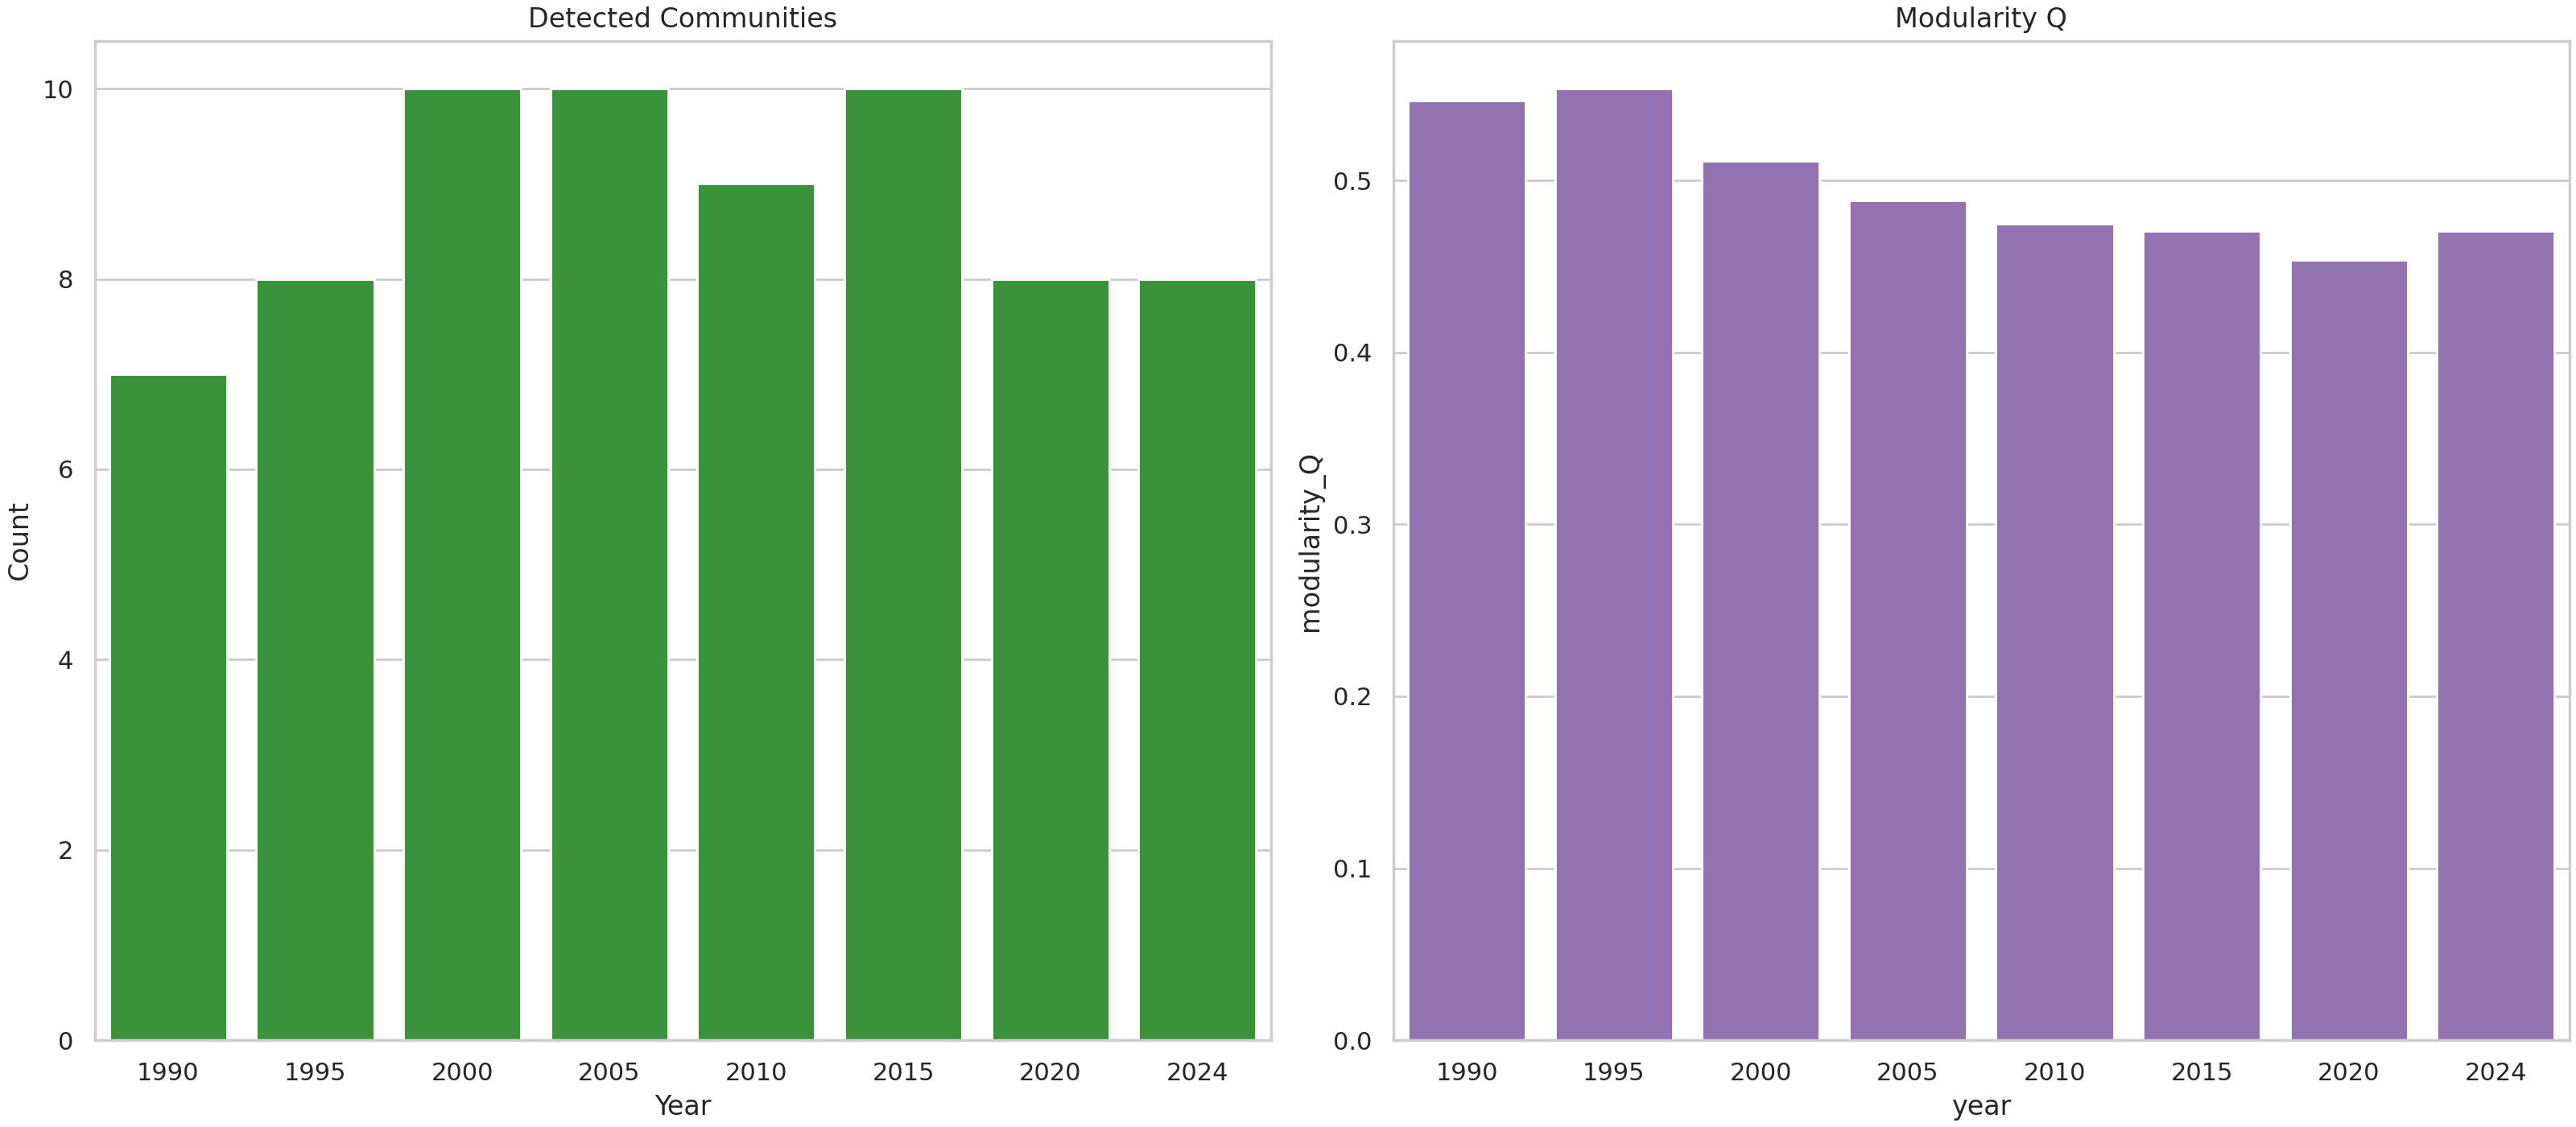
\includegraphics[width=0.8\textwidth]{deliverables_outputs/powerbi_exports/screenshots/dashboard_04_communities.png}
  \caption{Community Structure}
\end{figure}

\begin{figure}[h!]
  \centering
  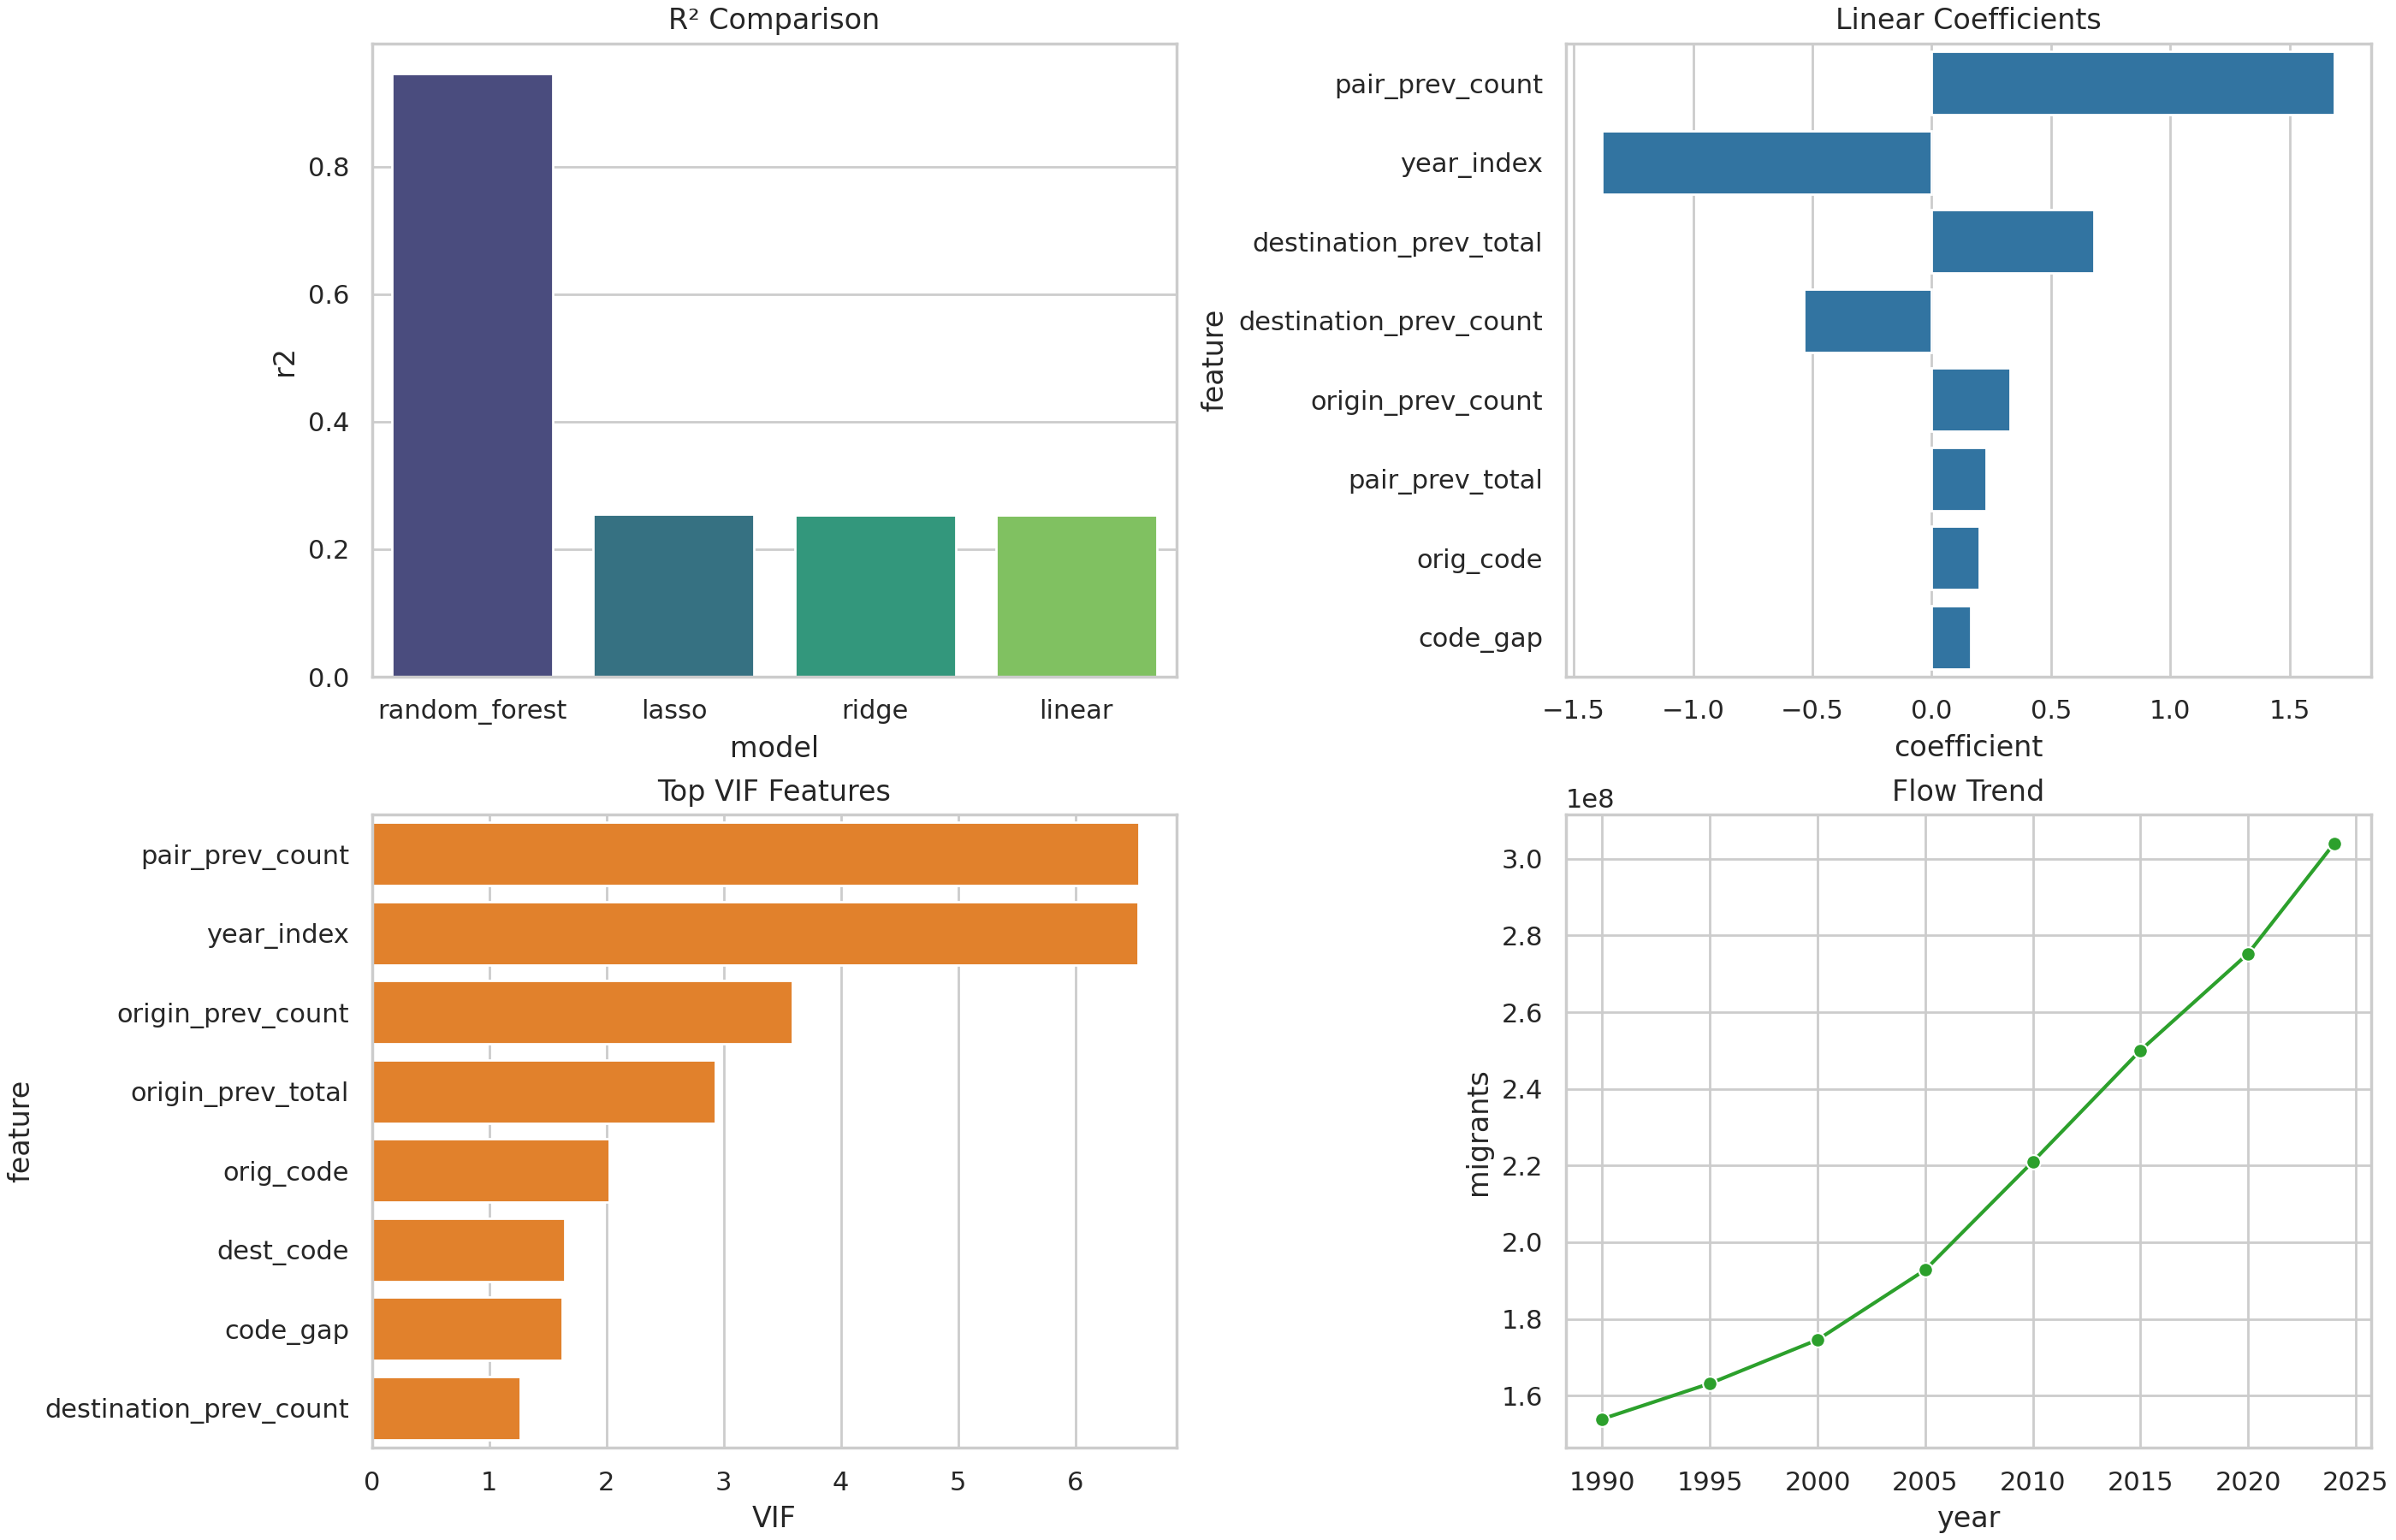
\includegraphics[width=0.8\textwidth]{deliverables_outputs/powerbi_exports/screenshots/dashboard_05_regression.png}
  \caption{Regression Diagnostics}
\end{figure}

\section{References}
\begin{itemize}
  \item United Nations, Department of Economic and Social Affairs. \textit{International Migrant Stock 2024}.
  \item World Bank Open Data
  \item Newman, M. E. J. (2010). \textit{Networks: An Introduction}. Oxford University Press.
  \item Blondel, V. D., Guillaume, J.-L., Lambiotte, R., \& Lefebvre, E. (2008). Fast unfolding of communities in large networks.
  \item Traag, V. A., Waltman, L., \& van Eck, N. J. (2019). From Louvain to Leiden: guaranteeing well-connected communities.
\end{itemize}

\end{document}
